\documentclass[a4project, twocolumn]{article}


\usepackage{parskip} % Package to tweak paragraph skipping
\usepackage{tikz} % Package for drawing
\usepackage{amsmath}
\usepackage{txfonts}
\usepackage{amssymb}
\usepackage[makeroom]{cancel}
\usepackage{hyperref}
\usepackage{fancyhdr}
\usepackage{enumerate}
\usepackage{graphicx}
\usepackage{wrapfig}
\graphicspath{ {images/} }
\usepackage{hyperref}
\usepackage[utf8]{inputenc}
\usepackage{color}
\usepackage[document]{ragged2e}
\usepackage{listings}


\usepackage[
style=authoryear,
citestyle=authoryear,
%autocite=superscript,
backend=biber
]{biblatex}
\addbibresource{MMR.bib}

% This command just to put the brackets in the book references
\DeclareCiteCommand{\supercite}[\mkbibsuperscript]
  {\usebibmacro{cite:init}%
   \let\multicitedelim=\supercitedelim
   \iffieldundef{prenote}
     {}
     {\Bibliographywarning{Ignoring prenote argument}}%
   \iffieldundef{postnote}
     {}
     {\Bibliographywarning{Ignoring postnote argument}}%
  \bibopenbracket}%
  {\usebibmacro{citeindex}%
   \usebibmacro{cite:comp}}
  {}
  {\usebibmacro{cite:dump}\bibclosebracket}
%end command


\newcommand{\Mod}[1]{\ (\text{mod}\ #1)}
\newcommand{\Atan}[1]{\arctan{\left( #1 \right)}}
\newcommand{\Para}[1]{\left( #1 \right)}
\newcommand{\Barr}[1]{\left| #1 \right|}

\newcommand{\Cos}[1]{\cos{\left( #1 \right)}}
\newcommand{\Coss}[1]{\cos^2{\left( #1 \right)}}
\newcommand{\Sin}[1]{\sin{\left( #1 \right)}}
\newcommand{\Sins}[1]{\sin^2{\left( #1 \right)}}
\usepackage{geometry}

\renewcommand{\theequation}{\thesection.\arabic{equation}}


 \geometry{
 a4paper,
 total={170mm,252mm},
 left=25mm,
 top=25mm,
 }


\pagestyle{fancy}
\fancyhf{}
\rhead{Predicting missing Data in InfoRM}

\rfoot{Page \thepage}
\lfoot{Joaqu\'in B\'ejar Garc\'ia}


\title{Predicting missing Data in InfoRM}
\author{Joaqu\'in B\'ejar Garc\'ia}
\date{23\textsuperscript{st} August 2017}


\begin{document}
\nocite{*}

\begin{titlepage}
	\centering

	\vspace{1.5cm}
	{\huge\bfseries Predicting missing Data in InfoRM \par}
	\vspace{1.5cm}
	
\includegraphics[width=0.75\textwidth]{INFORM_banner.png}\par\vspace{1cm}
	\vfill
	{\Large\itshape 
	Joaquín Béjar García \\
	{\fontfamily{cmtt}\selectfont
	\small{Joaquin.BEJAR-GARCIA@ext.ec.europa.eu}
	}
	\par}
\section{Abstract}
\justify
This project try to approach the moderns statistics methods to the current InfoRM development. We will try to show how different mathematical methods can deal with missed data further than to apply just imputation methods from existing predictors or variables. We will be able to predict values and fill the gaps on the indexes using the information available each year and country. These predictions come with a score or error to provide a level of accuracy to the model.

This project, as well as many others, use tools that take out current information, sift through data looking for patterns that are relevant to our problem, and return answers and error levels. The process of developing these kinds of tools has evolved throughout a number of fields such as chemistry, computer science, physics, and statistics and has been called "machine learning", "artificial intelligent", "pattern recognition", "data mining", "predictive analytic", and "knowledge discovery". While each field approaches the problem using different perspectives and tool sets, the ultimate objective is the same: to make an accurate prediction.

	\vfill

% Bottom of the page
	{\large \today\par}
\end{titlepage}
\thispagestyle{plain}
%\large
%\maketitle
\clearpage

\justify
\onecolumn
\Large{
\tableofcontents}

%\large{}
\normalsize
\vfill
\pagebreak
\twocolumn

\section{Introduction}

The main motivations for using these new methods in InfoRM, arise from the need to predict certain trends in countries that otherwise would not be possible due to the lack of information or parameters in the original data of certain countries. To achieve this, the objective is to find the maximum correlation between available information and the indicators not present.

Thanks to this new development, InfoRM will have information closer to reality and will be able to present more precise predictions and trends about each of the countries in its different Social-Economic areas.


\section{State of the Art}
INFORM is a global, open-source risk assessment for humanitarian crises and disasters. It can support decisions about prevention, preparedness and response. INFORM is a collaboration of the Inter-Agency Standing Committee Reference Group of Risk, Early Warning and Preparedness and the European Commission.

The Inter-Agency Standing Committee (IASC) is the primary mechanism for inter-agency coordination of humanitarian assistance. It is a unique forum involving the key UN and non-UN humanitarian partners. The IASC was established in June 1992 in response to United Nations General Assembly Resolution 46/182 on the strengthening of humanitarian assistance.

http://www.inform-index.org/

INFORM include Subnational models that are outside of the scope of this research.

\subsection{About InfoRM Data}

The information used in InfoRM come from different notoriety sources providing massive knowledge to the report, however due to its nature the raw data come with a big amount of gaps, creating some misinformation in the final results.

Current InfoRM data set include information from 67 (years) x 248 (countries) x 249 (indexes), mostly of the information belong to last 25 years.

\subsection{About the data}
We have used data sources from DataBankWorld Development Indicators, World Health Organization and InfoRM 2017 for this research, this databases provide a wide range of predictors which let us create several different data sets and therefore different models without change the models used. 

Main reason to use these sources is maximize the available information relative to each country and the correlation with the values to predict. As results of this union the dataset use in this research is 67 (years) x 248 (countries) x 507 Indexes. Adding more data to the data set we are adding more information to the predicted model and improving the future score of each indicator. The main goal of adding these data is not include them in the InfoRM methodology but increase the probability of having a better score in a indicator that in fact is used in the methodology.

Adding more data sometimes means add more noise, in this case Random Forest Regressor works as a filter removing that noise to a large degree.


The data set for this analysis can be found on the \href{https://TBDs}{InfoRM Repository}. For the purposes of this Analysis, no features will be excluded in the analysis.

\subsection{About the Predictive models}

Throughout the project we put focus in the missed indexes used in InfoRM and how the models provide information about it, however these models could be applied to any variable or predictor used in the data sources.

This research is based in the field of supervised learning and the area of numerical prediction more often called regression. The other area inside supervised learning is classification out of the scope of this project.

Other field inside of machine learning is Unsupervised Learning aka. Clustering which could provide an improvement in the research that will be include in future, is out of the scope of this project.


\newpage
\section{About Data Analysis}

Data analysis  is a process of inspecting, cleansing, transforming, and modeling data with the goal of discovering useful information, suggesting conclusions, and supporting decision-making. Data analysis has multiple facets and approaches, encompassing diverse techniques under a variety of names, in different business, science, and social science domains. Here we show some methods used to improve the quality of the process.

\subsection{Data Preparation}

The data for this process comes mainly in two formats and two different sources: The first come from the Database of InfoRM in MSSQL where the present information is stored without specifying where the missing data are. With this information a 3D array is created with axes year, country and indicator where the data not present is shown as NaN. On the other hand, another 258 new indicators are collected using the WHO and WorldBank as source, these indicators also present missing data in some of their indicators. As with the initial indicators, a 3D Array with axes year, country and indicator is created. Both arrays come together to create a unique array with which the prediction process begins.

\subsubsection{Missing Data}

The method of multiple imputation is motivated by the need to provide a approximated value that show the current status of a given country in a given predictor. We assume that the database is analyzed by several secondary analysts, with a wide range of inferential goals and using a variety of statistical software tools and methods well suited only for complete data. We apply a small number of alternative completions, based on a model for non response. We applied the complete-data method to each completed dataset. Then results are then averaged, with an appropriate inflation for the sampling variance that reflects the uncertainty about the missing values. 

\subsubsection{Lost information}

Imputation imply the loss of efficiency even that the first few imputations reduce the sampling variance substantially and latter imputations make only small contributions to the precision of the completed dataset.

The modelling and simulation steps guaranty that within and between imputation variances of the completed datasets accurately reflect the uncertainty about the missing values and it's unbiased.

\subsubsection{Data Cleaning}

Data cleaning is a common practice before to start building the a model, in our case we cannot take the risk to remove more information from the dataset. Random Forest helps in this task thanks to its good performance dealing with noise and outliers.
 
\subsubsection{Reducing Predictors}

Random forests, are useful for feature selection in addition to being effective regressors.  One approach to dimensional reduction is to generate a large and carefully constructed set of trees against a target attribute and then use each attribute’s usage statistics to find the most informative subset of features.  Specifically, we can generate a large set of very shallow trees, with each tree being trained on a small fraction of the total number of attributes. If an attribute is often selected as best split, it is most likely an informative feature to retain. A score calculated on the attribute usage statistics in the random forest tells us relative to the other attributes which are the most predictive attributes

\subsection{Data Exploration}

Familiarizing with the data through an exploratory process is a fundamental practice to help you better understand and justify our results. Since the main goal of this project is to construct a working model which has the capability of predicting the value of an index, we will need to separate the dataset into features and the target variables.

\subsubsection{Type of Variables}

Every predictor used in InfoRM are quantitative and continuous variables hence we deal with a regression problem. Random Forest is not too sensitive to outliers or no normalized distributions, if data is not normally distributed, especially if the mean and median vary significantly (indicating a large skew), it is most often appropriate to apply a non-linear scaling, particularly for financial data. One way to achieve this scaling is by using a Box-Cox test, which calculates the best power transformation of the data that reduces skewness.


\subsection{Outlier Detection}

Detecting outliers in the data is extremely important in the data preprocessing step of any analysis. The presence of outliers can often skew results which take into consideration these data points. There are many "rules of thumb" for what constitutes an outlier in a dataset. Here, we use Tukey's Method for identifying outliers: An outlier step is calculated as 1.5 times the interquartile range (IQR). A data point with a feature that is beyond an outlier step outside of the IQR for that feature is considered abnormal.

\section{Developing a Model}
 
\subsection{Maximize Entropy}

Entropy is the amount of information in a chosen data set. We assume the missing data do not provide information. Given a Country and a Series or indicator we have to take a sub data set where the entropy is maximum.

\begin{align*}
    ME_{\Para{C \times S}} &\triangleq Cor_{S} \times \{ \dim{D_{CS}}\colon \forall X_{ij} \notin \varnothing \}  
\end{align*}

Where $Cor_S$ is the matrix correlation of S and $D_{CS}$ is the matrix of elements not null in the subset of $C \times S$

 
\subsection{Performance Metric}

It is difficult to measure the quality of a given model without quantifying its performance over training and testing. This is typically done using some type of performance metric, whether it is through calculating some type of error, the goodness of fit, or some other useful measurement. For this project, we calculate the coefficient of determination, $R^2$, to quantify your model's performance. The coefficient of determination for a model is a useful statistic in regression analysis, as it often describes how "good" that model is at making predictions.

The values for $R^2$ range from 0 to 1, which captures the percentage of squared correlation between the predicted and actual values of the target variable. A model with an R2 of 0 always fails to predict the target variable, whereas a model with an R2 of 1 perfectly predicts the target variable. Any value between 0 and 1 indicates what percentage of the target variable, using this model, can be explained by the features. A model can be given a negative R2 as well, which indicates that the model is no better than one that naively predicts the mean of the target variable.

\subsection{Overfitting}

Overfitting is one critical problem that may make the results worse, but for Random Forest algorithm, if there are enough trees in the forest, the classifier won’t overfit the model. The advantage is the classifier of Random Forest can handle missing values.

\subsection{Error}

The error is the measure that tell us how wrong is the prediction in its average. We use the following method to calculate the Mean Square Error in the data set after predictions have been made.

\begin{align*}
    E_S &= \dfrac{1}{\dim{(S)}}\sum^{\varphi_n}_{i=\varphi_0} \Para{\hat{y}_i-y_i}^2\\
    E_C &= \dfrac{1}{\dim{(C)}} \sum^{\nu_n}_{k=\nu_0} E_{s_k}\\
    &= \dfrac{1}{\dim{(S \times C)}} \sum^{\nu_n}_{k=\nu_0} \sum^{\varphi_n}_{i=\varphi_0}  \Para{\hat{y}_{ik}-y_{ik}}^2 
\end{align*}
Where $m$ is the number of years in observations and $n$ is the number of series, $S$ is the vector of Series and $C$ the vector of countries

\subsection{$R^2$ Scoring}

$R^2$ is the proportion of the variance in the outputs that is predictable from the input variables, express how the hypothesis function fits the dataset.

\begin{align*}
    \bar{y} &= \dfrac{1}{n} \sum^{n}_{j=1} y_j\\
    n\sigma^2 &= \sum^{n}_{i=1}\Para{y_i - \bar{y}}^2\\
    R^2 &\equiv 1 - \dfrac{\sum^{n}_{i=1}\Para{y_i-\hat{y}_i}^2}{n\sigma^2}\\
    R^2_S &\equiv 1 - \sum^{\varphi_n}_{i=\varphi_0}  \dfrac{\Para{y_i-\hat{y}_i}^2}{n\sigma^2}\hspace{15pt} \forall \varphi \in S\\
    R^2_C &\equiv \dfrac{1}{\dim{(C)}} \sum^{\nu_n}_{k=\nu_1} R^2_{s_k}\hspace{15pt}\forall \nu \in C\\
    R^2_C &\equiv \dfrac{1}{\dim{(C)}} \sum^{\nu_n}_{k=\nu_1} \Para{1 - \sum^{\varphi_n}_{i=\varphi_0} \dfrac{\Para{y_{ik}-\hat{y}_{ik}}^2}{n \sigma^2} }
\end{align*}

$R^2$ does not indicate whether the predictors are a cause of the changes in the dependent variable, we used the correlation function to measure this as well as  collinearity present in the data on the explanatory variables. This measure does not show if a omitted-variable bias exists or if we use the correct regression method.

$R^2$ does not indicate if the most appropriate set of independent variables has been chosen, we use the max entropy for this. 

The model might be improved by using transformed versions of the existing set of independent variables but $R^2$ is not a indicative of this. $R^2$ does not show if there are enough data points to make a solid conclusion.

\subsection{Shuffle and Split Data}

The data is also shuffled into a random order when creating the training and testing subsets to remove any bias in the ordering of the dataset.

\subsection{Training and Testing}

If we don't split the data, we risk having a model that can only make good predictions with the training data set, hence, we would end up with an overfit model.

\section{Analyzing Model Performance}

Looking several models' learning and testing performances on various subsets of training data. Additionally, we investigate one particular algorithm with an increasing 'max depth' parameter on the full training set to observe how model complexity affects performance. Graphing the model's performance based on varying criteria is beneficial in the analysis process, such as visualizing behavior that may not have been apparent from the results alone.

A 'Random Forest Regressor' usually has a better generalization performance than an individual decision tree due to randomness that helps to decrease the model variance. Other advantages of RF are that they are less sensitive to outliers in the dataset and don't require much parameter tuning. The only parameter in RF that we typically need to experiment with is the number of trees in the ensemble and the max depth of the trees. The RF algorithm is almost identical to RF algorithm for classification, the only difference is that we use MSE criterion to grow the individual decision trees, and the predicted target variable is calculated as the average prediction over all decision trees.

\subsection{Learning Curves}

Each graph visualizes the learning curves of the model for both training and testing as the size of the training set is increased. Note that the shaded region of a learning curve denotes the uncertainty of that curve (measured as the standard deviation). The model is scored on both the training and testing sets using $R^2$, the coefficient of determination.  

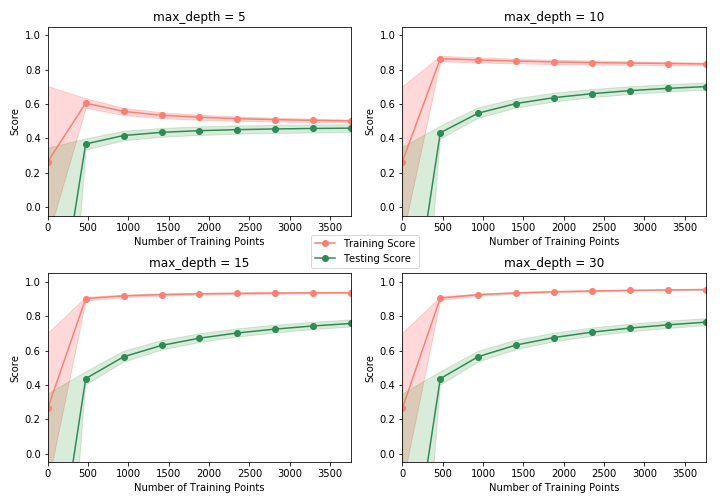
\includegraphics[width=0.50\textwidth]{ModelLearning}\par\vspace{1cm}\label{p1}

\subsection{Complexity Curves}

The graph produces two complexity curves, one for training and one for validation. Similar to the learning curves, the shaded regions of both the complexity curves denote the uncertainty in those curves, and the model is scored on both the training and validation sets using the performance metric function. The shaded regions of both the complexity curves denote the uncertainty in those curves, and the model is scored on both the training and validation sets.

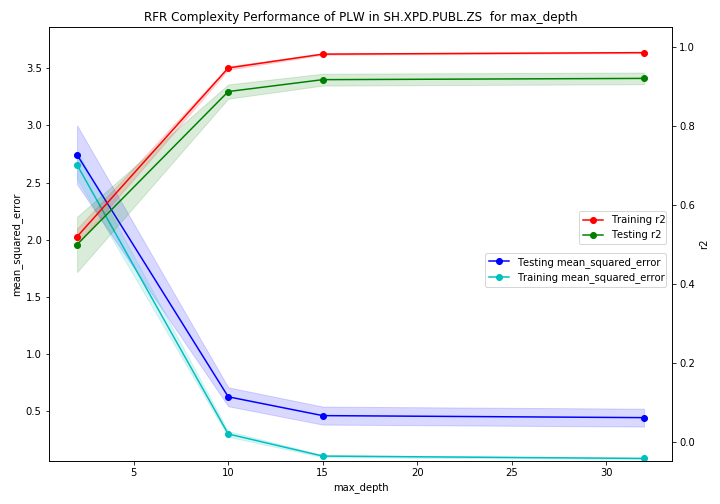
\includegraphics[width=0.50\textwidth]{ModelComplexity01}\par\vspace{1cm}\label{p2}

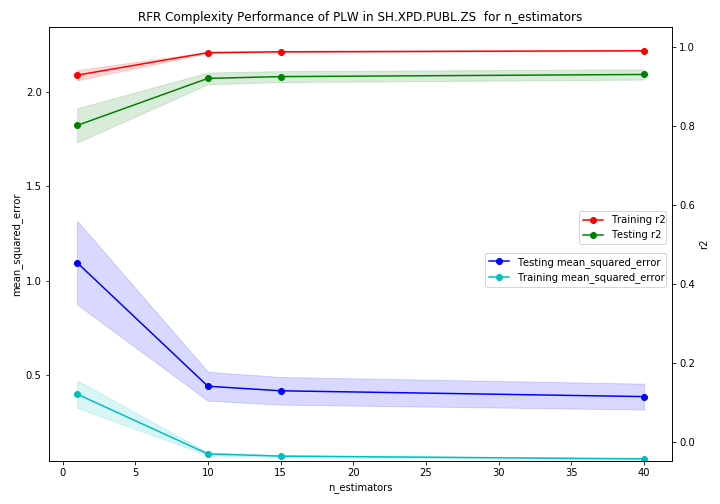
\includegraphics[width=0.50\textwidth]{ModelComplexity02}\par\vspace{1cm}\label{p3}

\subsection{Bias-Variance Trade-off}

The bias-variance trade-off is a central problem in supervised learning. Ideally, one wants to choose a model that both accurately captures the regularities in its training data, but also generalizes well to unseen data. Unfortunately, it is typically impossible to do both simultaneously. High-variance learning methods may be able to represent their training set well, but are at risk of overfitting to noisy or unrepresentative training data.
In contrast, algorithms with high bias typically produce simpler models that don't tend to overfit, but may underfit their training data, failing to capture important regularities.

When the training and testing errors converge and are quite high this usually means the model is biased. No matter how much data we feed it, the model cannot represent the underlying relationship and therefore has systematic high errors.

When there is a large gap between the training and testing error this generally means the model suffers from high variance. Unlike a biased model, models that suffer from variance generally require more data to improve. We can also limit variance by simplifying the model to represent only the most important features of the data.

\subsection{Best-Guess Optimal Model}

In the above example, maximum depth of 15 is the Ideal Learning Curve: The ultimate goal for a model is one that has good performance that generalizes well to unseen data. In this case, both the testing and training curves converge at similar values. The smaller the gap between the training and testing sets, the better our model generalizes. The better the performance on the testing set, the better our model performs.

\section{Evaluating Model Performance}

\subsection{Grid Search}

We use $Grid\ Search$ as a way of systematically working through multiple combinations of parameter tunes, cross-validating as it goes to determine which tune gives the best performance. The $fit$ function tries all the parameter combinations, and returns a fitted classifier that's automatically tuned to the optimal parameter combination. We access the parameter values via the classifier.

A grid search algorithm guides by the performance metric and measure by cross-validation on the training set. Fine tuning a learning algorithm is a more successful learning/testing performance in terms of the application for grid search.

As we have used Random Forest Regressor the main tuning parameters that have been searched are $Max\ Depth$ of trees ($M$) and $Number\ of\ trees$ to use ($N$). Each series or indicator have their own shape, size and property which means that we cannot use a common set of parameters in the fitting.

Dealing with the issue of finding the best tuning parameters for each series, have to avoid to increase the complexity of the model giving a wide range of search in $M$ and $N$. We tacked this issue giving random values to M and N in first instance. After several iteration the output of the model creates a dataset of performance metrics that we use to find the best parameters per series, given the size of the matrix.

Table \ref{tab:a} show an example about how the model works using random values in $M$ and $N$, later on we will use this new dataset to build a linear regression model in charge of find the best range of $M$s and $N$s to pass these as parameters to Grid Search.

\begin{table*}
  \centering
  \begin{tabular}{@{}l|l|rrrrrrr@{}}
        Country & Series & $R^2$ & MSE & X & Y & Time (s) & $M$ & $N$ \\ \hline
        EAR & HLT.SH.MED.PHYS.ZS & 0.316 & 33.048 & 84 & 4 & 32.4 & 10 & 16 \\ 
        EAP & HLT.SH.TBS.INCD & 0.413 & 14.335 & 32 & 22 & 11.7 & 12 & 6 \\ 
        DMA & IDP\_B & 0.000 & 313629.374 & 59 & 9 & 13.3 & 12 & 16 \\ 
        DOM & H\_Pandemic & 0.870 & 0.630 & 124 & 5 & 30.1 & 12 & 16 \\
        EAR & HLT.SH.TBS.INCD & 0.424 & 14.198 & 32 & 22 & 13.0 & 8 & 6 \\
        CHN & H\_Climate & 0.000 & 2.303 & 61 & 8 & 19.1 & 13 & 13 \\ 
        CPV & H\_Pandemic & 0.870 & 0.630 & 124 & 5 & 31.2 & 12 & 16 \\
        CHL & H\_Pandemic & 0.870 & 0.630 & 124 & 5 & 33.7 & 12 & 16 \\
        DOM & IDP\_B & 0.000 & 214827.213 & 59 & 9 & 13.4 & 9 & 16 \\ 
        DZA & HLT.SH.MED.PHYS.ZS & 0.000 & 33.108 & 104 & 20 & 39.9 & 12 & 17 
  \end{tabular}
  \caption{Sample learning dataset with Random $M \in [5,16]$ and $N \in [5,18]$}\label{tab:a}
\end{table*}

\subsection{K-Fold Cross-Validation}
Hence the K-Fold Cross-Validation $\Para{CV}$ estimate of prediction error:

\begin{align*}
CV\Para{\hat{f}}= \dfrac{1}{N} \sum_{i=1}^{N}L\Para{y_i,\hat{f}^{-k(i)}\Para{x_i}}
\end{align*}

Where $\hat{f}^{-k(i)}\Para{x_i}$ denotes the $i$th fitted function with $k$th part of the dataset removed

\subsection{Fitting a Model}

Our final implementation requires to bring everything together and train a model using the decision tree algorithm. To ensure that we produce an optimized model, we train the model using the grid search technique to optimize the $'max\_depth'$ parameter for the decision tree. The $'max\_depth'$ parameter can be thought of as how many questions the decision tree algorithm is allowed to ask about the data before making a prediction. 

\section{Making Predictions}

Once a model has been trained on a given set of data, it can now be used to make predictions on new sets of input data. In the case of a Random Forest Regressor, the model has learned what the best questions to ask about the input data are, and can respond with a prediction for the target variable. We use these predictions to gain information about data where the value of the target variable is unknown, such as data the model was not trained on.

\subsection{Optimal Model}

As we have seen in the complexity curves, the optimal model is always linked to the complexity and some times the price we have to pay for a perfect model require infinity computational resources or time, which is not feasible in a practical environment. Find a optimal model is a never ending process that always finish under the analyst supervision, last score in this model is 88\% accuracy, an improves of just 1\% in the model require 1 month of computation.

\subsection{Predicting Index}

It's very important do not fall into temptation to get the predicted values as real, these predicted indexes are statistical values and they should be taken as it. As well as imputation that try to show values close to the real ones, but thanks to supervised learning we can provide values of how far or how accurate they are.

\subsection{Sensitivity}

An optimal model is not necessarily a robust model. Sometimes, a model is either too complex or too simple to sufficiently generalize to new data. Sometimes, a model could use a learning algorithm that is not appropriate for the structure of the data given. Other times, the data itself could be too noisy or contain too few samples to allow a model to adequately capture the target variable, for example the model is underfitted. $R^2 \text{ and } MSE$ are the parameters in charge to define the level of quality of our model.

\subsection{Applicability}

How relevant today is data that was collected from 1978?: Those data would be out of date, indexes have changed a lot during last almost 40 years and areas that in 1978 have a specific statistics, nowadays could be totally different.

Are the features present in the data sufficient to describe a missing value?: Other features should be included to predict those indexes more accuracy, for example, more sources.

\section{Results}

The main objective of this exercise was to have indicators in each country per year, these values would show trends that simple imputation could not show. As a result, a series of raw data is available that replaces the old gaps in such a way that by amplifying InfoRM's own methodology, a new report is created that tries to show results closer to reality.\textbf{ It's really important to keep in mind that predicted values are not real values}, in some cases $R^2=0$ that means the predicted value is totally random and should be taken as is. This is due the none correlation with other indicators or too much noise. In other cases the \textit{Mean Square Error} could be too high or with high variance therefore the range of predicted values result too wide.

Predicted indicators are included in the InfoRM methodology like the real values, their don't require a special treatment, but R2 and MSE must be included.  

\subsection{Model Comparison}
The final goal is to compare the previous model with the new one. We use real vs predicted values to visually show the results, following plot shows an example of how the new model is closer to the perfect line.

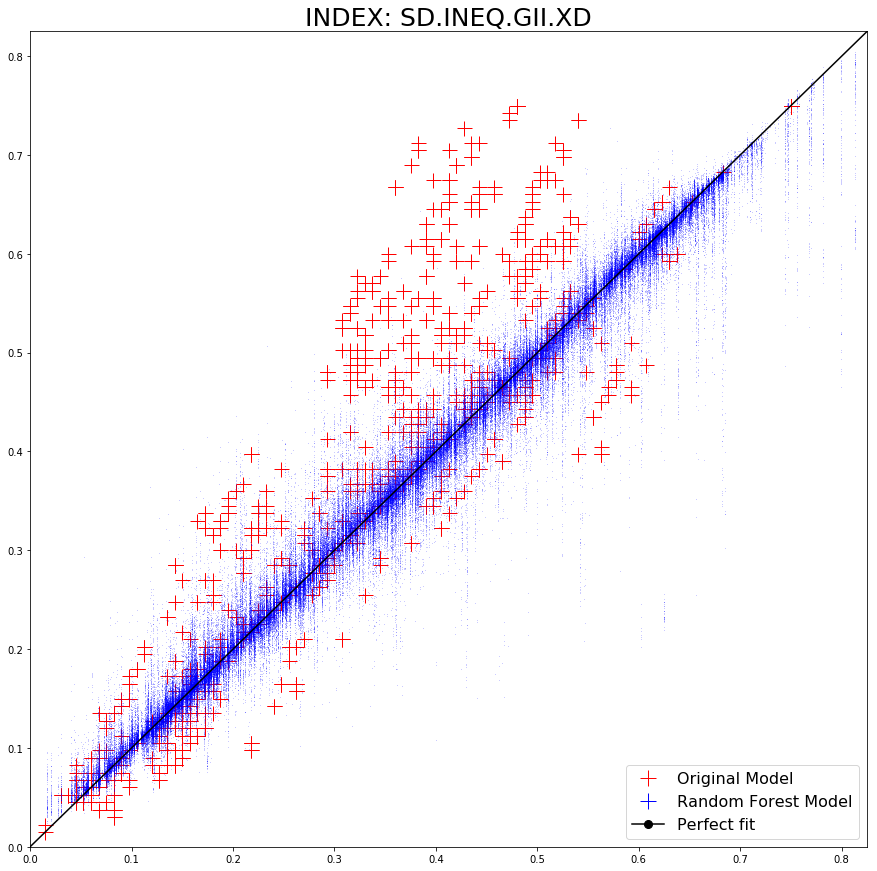
\includegraphics[width=0.50\textwidth]{model_comparison.png}\par\vspace{1cm}\label{p3}



\onecolumn

 


\printbibliography[title={References}]
\end{document}

